\section{Data Analysis}

\subsection{IV Characterstics of\\Silicon Diode (IN4148)}

    \begin{figure}[H]
     \centering
     \begin{subfigure}[b]{0.45\textwidth}
         \centering
         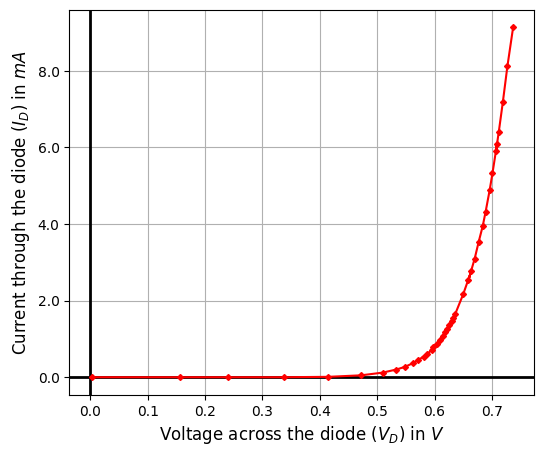
\includegraphics[width=\textwidth]{images/1.png}
         \caption{Si diode under forward bias}
         \label{fig1}
     \end{subfigure}
     \hfill
     \begin{subfigure}[b]{0.45\textwidth}
         \centering
         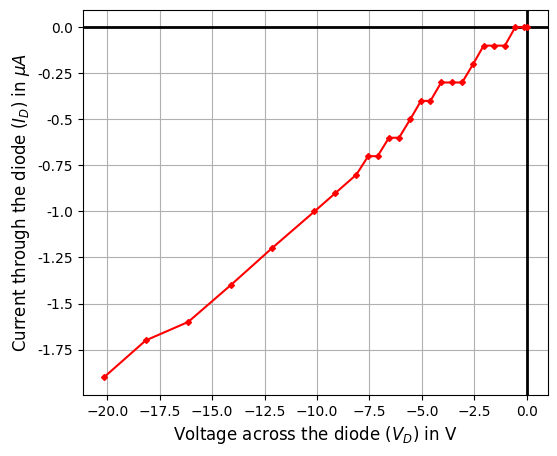
\includegraphics[width=\textwidth]{images/2.png}
         \caption{Si diode under reverse bias}
         \label{fig2}
     \end{subfigure}
     \hfill
        \caption{I-V characteristics graph of a Silicon Diode. The knee voltage is 0.65V but the breakdown voltage could not be detected. Note that the scale of y-axis in plot (b) is 3 order of magnitude less that plot (a), i.e. there is negligible current flowing through the diode under reverse bias.}
        \label{f1}
\end{figure}
\vspace{80pt}
\subsection{IV Characterstics of\\Zener Diode (C3V3PH)}

    \begin{figure}[H]
     \centering
     \begin{subfigure}[b]{0.45\textwidth}
         \centering
         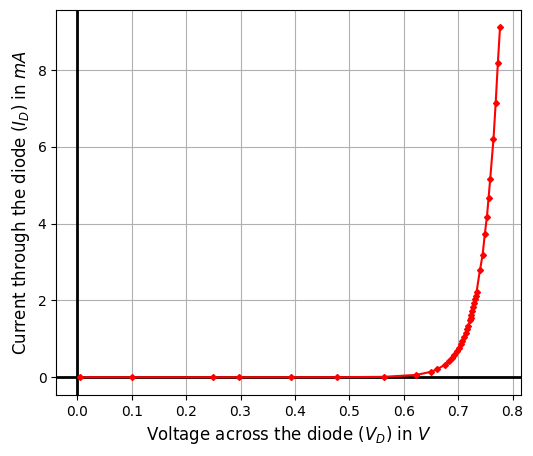
\includegraphics[width=\textwidth]{images/3.png}
         \caption{Zener diode under forward bias}
         \label{fig1}
     \end{subfigure}
     \hfill
     \begin{subfigure}[b]{0.45\textwidth}
         \centering
         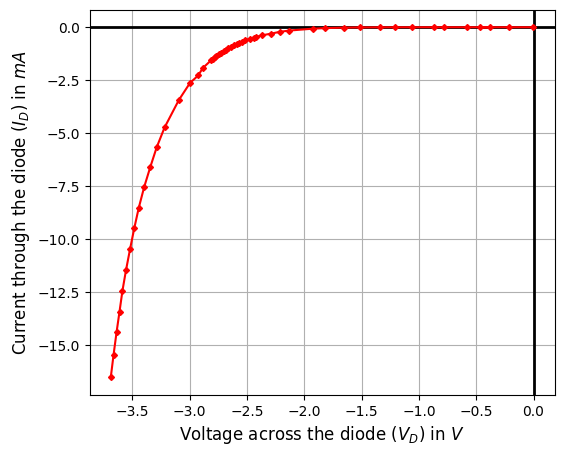
\includegraphics[width=\textwidth]{images/4.png}
         \caption{Zener diode under reverse bias}
         \label{fig2}
     \end{subfigure}
     \hfill
        \caption{I-V characteristics of the Zener Diode. The knee voltage is approximately 0.68V and the breakdown voltage is approximately 2.5V}
        \label{f1}
\end{figure}

\subsection{Calculations}
We can see from Fig 1(a) that the operating point point of the diode may lie somewhere above 0.72V. Let's take approximately $V_D = 0.727V$. 

Static resistance at $0.727V$,

\begin{align*}
    R_D &= \frac{V_D}{I_D}\\
    &= \frac{0.727}{8.12\cross10^-3} = 89.53\Omega
\end{align*}


Similarly, dynamic resistance at $0.727V$,

\begin{align*}
    r_D &= \frac{\Delta V_D}{\Delta I_D}\\
    &= \frac{0.727-0.719}{(8.12-7.18)\cross10^-3} \\
    &=8.51 \Omega
\end{align*}
